%!TEX root = ../main.tex
\section{Homework \thesection}

\subsection{Simple Fully-connected Neural Network}
We discussed neural networks in the class. In this problem, we will implement very simple fully-connected neural network. Here is
an example of 2-layer neural network.

We will use this model to the MNIST dataset.
As you all know, each image of MNIST is of \(28 \times 28\), and it contains a single hand-written digit.
If we vectorize it, it will be 784 vector.
We will use the notation \(x\) to represent this input vector.
The hidden layer consists of 50 neurons, and the output layer has 10 neurons.
The final output is a score vector, of which element represents a probability of each digit.
That is, \(s^{(1)}\) represents the probability of \(x\) being digit 0, \(s^{(2)}\) is for 1, \(\cdots, s^{(10)}\) is for 9.
If we train the model with the input vectors and the corresponding labels, the model can be used to predict which digit the given image contains from 0 to 9.
Now, go to \href{./hw6/p1.m}{\texttt{p1.m}}.
\begin{enumerate}
    \item First of all, implement the sigmoid function by filling up \href{./hw5/sigmoid.m}{\texttt{sigmoid.m}}.
    Then, fill in the blanks of \href{./hw6/p1.m}{\texttt{p1.m}}, with in the comment ``FILL THIS UP WITH YOUR CODE''.
    Remind that each output is just the weighted sum with the bias applied with some activation function.
    Include the code in the pdf report and submit your \href{./hw6/p1.m}{\texttt{p1.m}} to the Canvas.
    \item Now, run the code.
    It will give you two plots.
    The first one is the loss graph, and the other one is accuracy graph.
    Attach your plots and report the last test accuracy.
    \item How many ``learnable'' parameters (all the weights and bias) are there in this network?
    Get the number and report it.
\end{enumerate}
\subsubsection{Implementation}
\lstinputlisting[style=Matlab-editor]{./hw6/sigmoid.m}
\lstinputlisting[style=Matlab-editor]{./hw6/p1.m}
\subsubsection{Loss and Accuracy}
The last test accuracy is 95\%.
Figures are shown in \ref{fig:25}.
\begin{figure}[htbp]
	\centering
	\begin{subfigure}[t]{0.8\textwidth}
	    \centering
        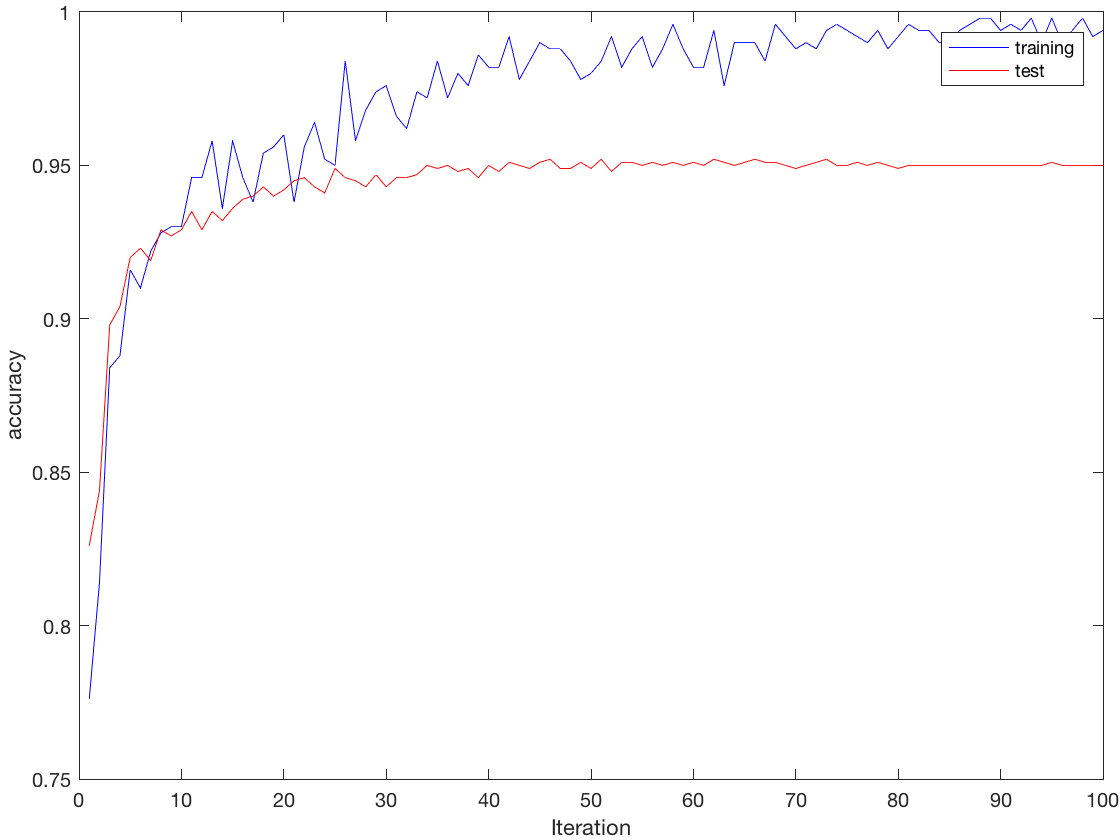
\includegraphics[width=\textwidth]{hw6/accuracy1.png}
		\caption{Accuracy}\label{fig:25a}
	\end{subfigure}
	\begin{subfigure}[t]{0.8\textwidth}
	    \centering
		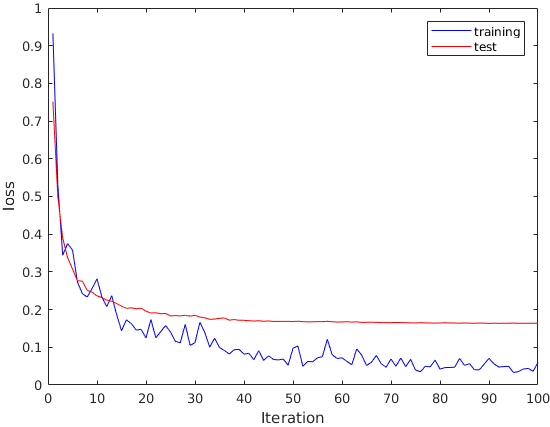
\includegraphics[width=\textwidth]{hw6/loss1.png}
		\caption{Loss}\label{fig:25b}
	\end{subfigure}
	\caption{Simple Fully-connected Neural Network Accuracy and Loss}\label{fig:25}
\end{figure}

\subsubsection{Learnable Parameters}
Total parameters: 39760.
\begin{align*}
    \texttt{size}(w_1)&=50\times784\\
    \texttt{size}(w_2)&=10\times50\\
    \texttt{size}(b_1)&=50\times1\\
    \texttt{size}(b_2)&=10\times1
\end{align*}

\newpage
\subsection{3-layer Neural Network}
Let's add one more hidden layer.
Then, our network will be 3-layer neural network.
Repeat the tasks.
\begin{enumerate}
    \item Fill in the blanks of \href{./hw6/p2.m}{\texttt{p2.m}}, with in the comment ``FILL THIS UP WITH YOUR CODE''.
    Note that we use Xaxier's scaling factor.
    Include the code in the pdf report and submit your \href{./hw6/p2.m}{\texttt{p2.m}} to the Canvas.
    \item Now, run the code.
    It will also give you two plots, which are the loss graph and the accuracy graph.
    Attach your plots and report the last test accuracy.
    \item How many ``learnable'' parameters (all the weights and bias) are there in this network?
    Get the number and report it.
\end{enumerate}
\subsubsection{Implementation}
\lstinputlisting[style=Matlab-editor]{./hw6/p2.m}
\subsubsection{Loss and Accuracy}
The last test accuracy is 94.8\%.
Figures are shown in \ref{fig:26}.
\begin{figure}[htbp]
	\centering
	\begin{subfigure}[t]{0.8\textwidth}
	    \centering
        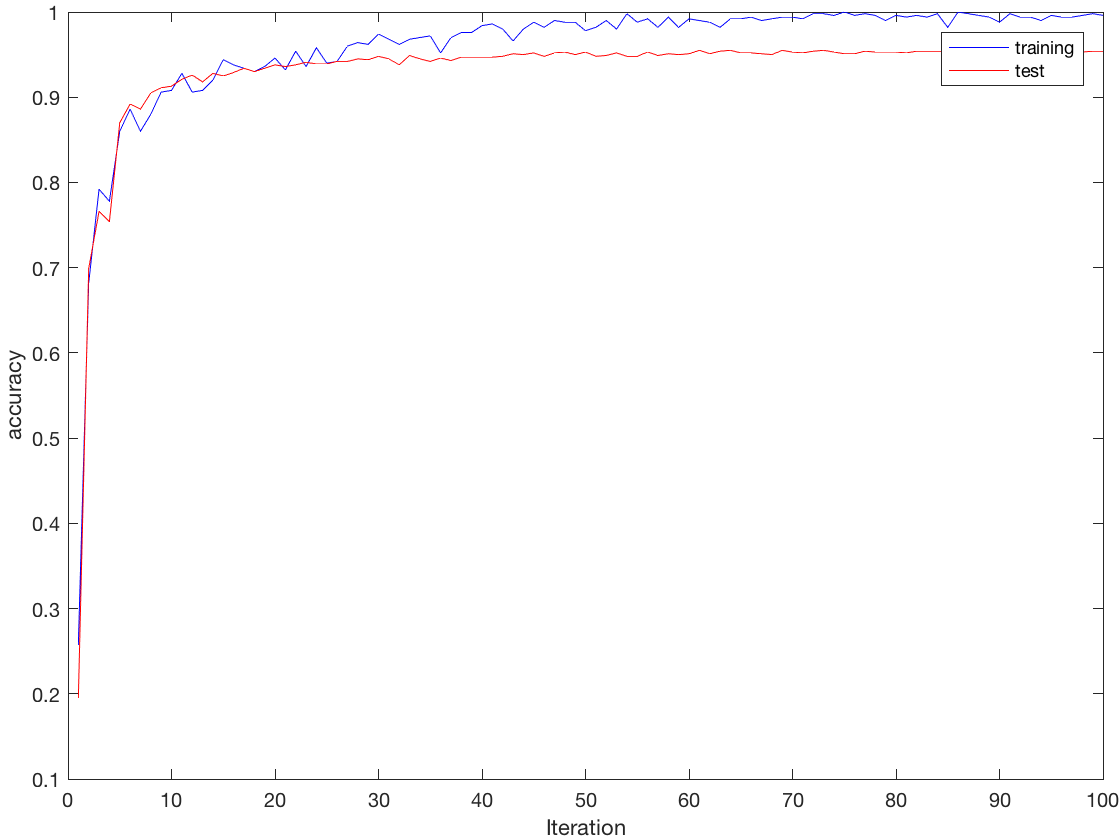
\includegraphics[width=\textwidth]{hw6/accuracy2.png}
		\caption{Accuracy}\label{fig:26a}
	\end{subfigure}
	\begin{subfigure}[t]{0.8\textwidth}
	    \centering
		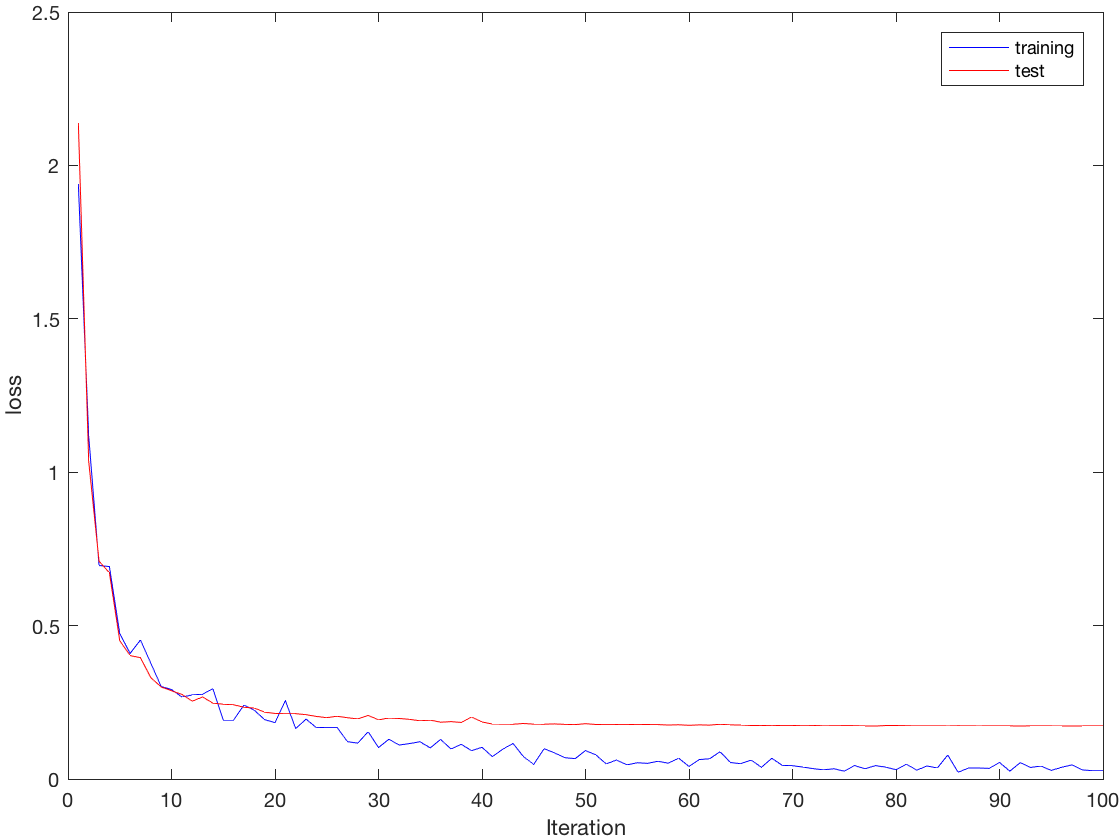
\includegraphics[width=\textwidth]{hw6/loss2.png}
		\caption{Loss}\label{fig:26b}
	\end{subfigure}
	\caption{3-layer Neural Network Accuracy and Loss}\label{fig:26}
\end{figure}
\subsubsection{Learnable Parameters}
Total parameters: 41090.
\begin{align*}
    \texttt{size}(w_1)&=50\times784\\
    \texttt{size}(w_2)&=30\times50\\
    \texttt{size}(w_3)&=10\times30\\
    \texttt{size}(b_1)&=50\times1\\
    \texttt{size}(b_2)&=30\times1\\
    \texttt{size}(b_3)&=10\times1
\end{align*}



\newpage
\subsection{Simple Convolutional Neural Network}
Pixels of natural images are highly spatially correlated.
Also, they are usually spatially stationary, which means that they can have common basis.
In this perspective, neurons are only locally connected to the previous input in the convolution layer, which is not the case of the fully connected layers.
In this problem, we will consider CNN with only a single convolution layer and fully connected layer.
The detailed information of this network is in \href{./hw6/p3.m}{\texttt{p3.m}}.
\begin{enumerate}
    \item Fill in the blanks of \href{./hw6/p3.m}{\texttt{p3.m}}, with in the comment ``FILL THIS UP WITH YOUR CODE''.
    Include the code in the pdf report and submit your \href{./hw6/p3.m}{\texttt{p3.m}} to the Canvas.
    \item Now, run the code.
    It will be really slow.
    I recommend to test your code with lower number of epochs (or lower number of training data).
    It will give you two plots.
    The first one is the loss graph, and the other one is accuracy graph.
    Attach your plots and report the last test accuracy.
    \item How many ``learnable'' parameters (all the weights and bias) are there in this network?
    Get the number and report it.
    \item Even if this network is really simple, it takes long time to be well trained.
    Describe simply why the GPU is necessary for deep neural networks.
\end{enumerate}
\subsubsection{Implementation}
\lstinputlisting[style=Matlab-editor]{./hw6/p3.m}
\subsubsection{Loss and Accuracy}
The last test accuracy is 92.1\%.
Figures are shown in \ref{fig:27}.
\begin{figure}[htbp]
	\centering
	\begin{subfigure}[t]{0.8\textwidth}
	    \centering
        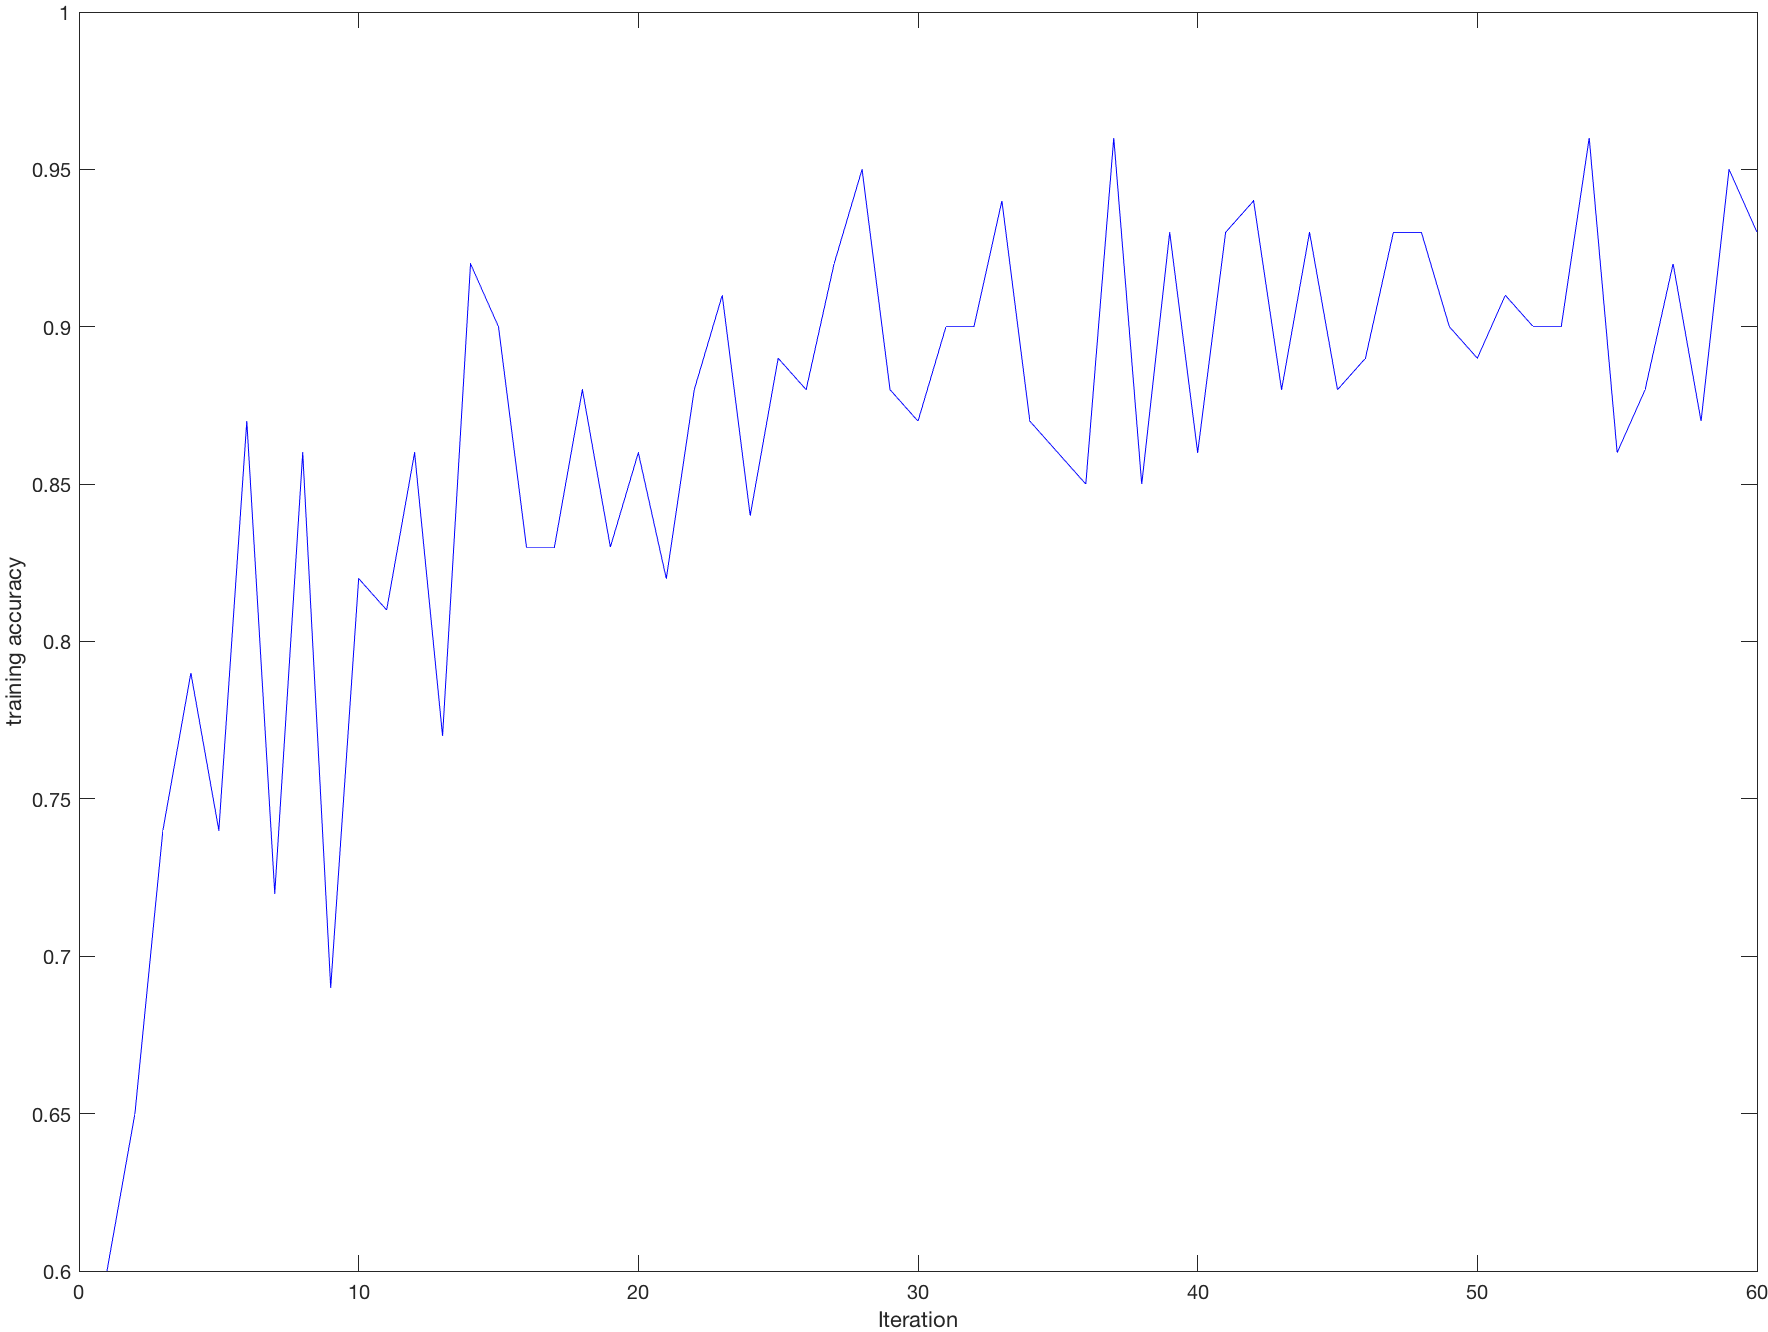
\includegraphics[width=\textwidth]{hw6/accuracy3.png}
		\caption{Accuracy}\label{fig:27a}
	\end{subfigure}
	\begin{subfigure}[t]{0.8\textwidth}
	    \centering
		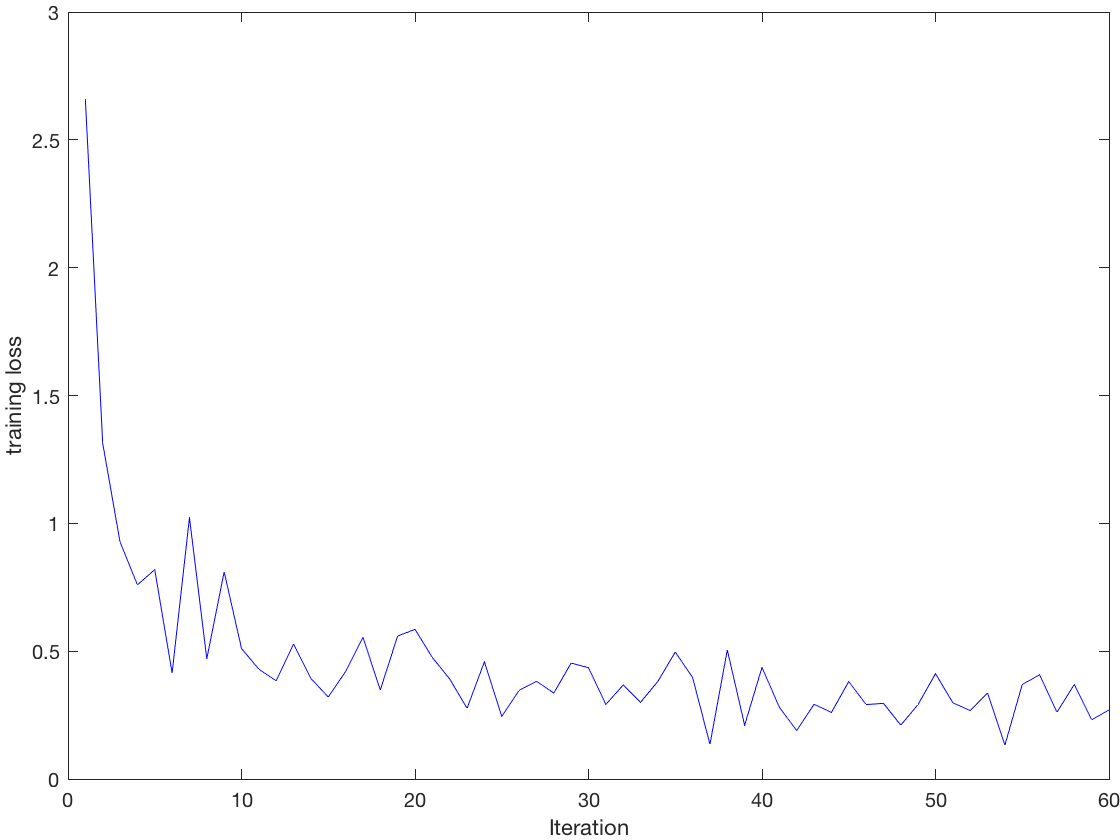
\includegraphics[width=\textwidth]{hw6/loss3.png}
		\caption{Loss}\label{fig:27b}
	\end{subfigure}
	\caption{Convolutional Neural Network Accuracy and Loss}\label{fig:27}
\end{figure}

\subsubsection{Learnable Parameters}
Total parameters: 29410.
\begin{align*}
    \texttt{size}(w)&=10\times2940\\
    \texttt{size}(b)&=10\times1
\end{align*}

\subsubsection{GPU Requirement}
In the \hyperref[profile]{Profile Summary}, we can see that these functions are called millions of times.
\begin{table}
    \centering
    \begin{tabular}{l|r|r|r}
        Function Name & Calls & Total Time & Self Time\\ \hline
        p3 & 1 & 754.505 s & 466.481 s\\
        kron & 9000000 &135.276 s & 135.276 s\\
        sigmoid & 9015000 & 104.339 s & 104.339 s\\
        rot90 & 9000000 & 37.339 s & 37.339 s\\
        squeeze & 9015000 & 10.836 s & 10.836 s\\
    \end{tabular}
    \label{profile}
    \caption{Profile Summary on \href{./hw6/p3.m}{\texttt{p3.m}}}
\end{table}
The computation of these functions are highly parallelizable, and doesn't require the branch structure such as \texttt{if...else..} statement.
Only float number multiplication and addition are required.
This is can be parallely done on GPUs, which has thousands of units that compute the float number operation.
This is much faster than using only CPU to do the calculation.